\section{Underlying modeling technique}
\label{section:contribution_0}

Our approach is based on emergent property estimation techniques \cite{hackenberg2012towards} and uses a model-based approach for validating requirements in early phases of system development proposed in \cite{hackenberg2014rapid}. An adaption to the ITS domain of this modeling technique was proposed in \cite{ascher2014early}, which facilitates the formulation of multi-objective traffic flows as an optimal control problem consisting of state variables, control variables, constraints and objectives. The approach employs a generic solver for system behavior estimation, which utilizes stochastic optimization techniques.

The proposed modeling technique employs the concept of components to break down complex problems into smaller pieces to be able to solve them more easily. For one, components are described by their behavior, i.e. the reachable state space. Furthermore, components are described by their ports and directed connections, i.e. channels between the ports of components. An overview of the meta-model of the approach is given in Figure~\ref{fig:meta_model}.

\begin{figure}[h]
	\centering
	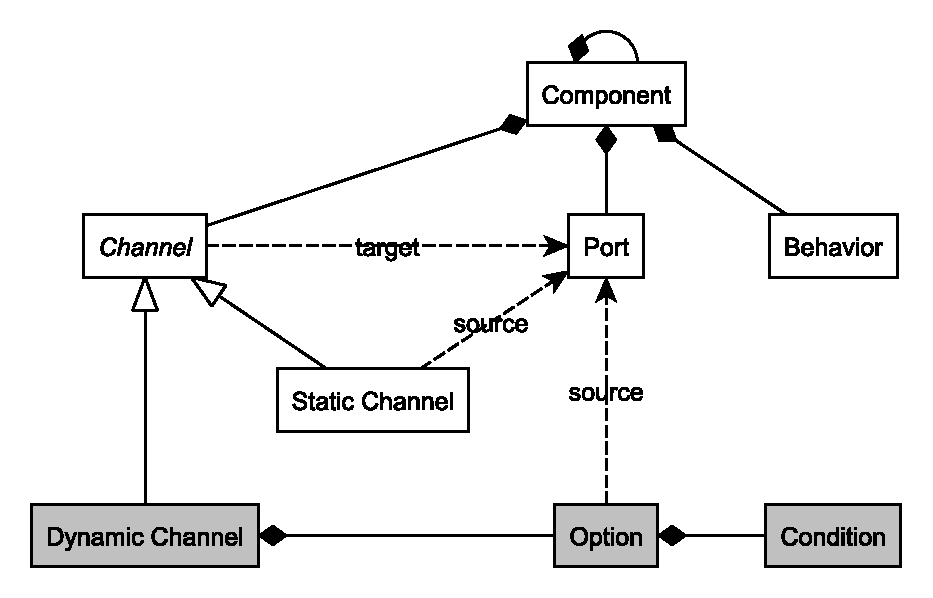
\includegraphics[width=\columnwidth]{../gfx/meta_model2.pdf}
	\caption{Meta-model of the underlying modeling technique extended with the concept of dynamic channels.}
	\label{fig:meta_model}
\end{figure}

In terms of their structure, model components can be either atomic or composed by other components. Ports can either represent input or output ports, and allow observations about specific behavior. Channels, i.e. directed connections between input and output ports, allow the modeling of interactivity between different components. Channels can either be static or dynamic. Static channels are bound to a specific source and target port. In contrast, dynamic channels are bound to a specific source port, but possess an option which determines the target port. In return, all possible target ports and their options also have to be registered to the dynamic channel. For dynamic channel evaluation, options encode conditions, which have to be fulfilled by both source and target port options. In case the condition of the source option is met by at least one target option, a single connection between a source and a target port exists. In case the condition of the source option isn't met by at least one target option or the target port of a applicable target option is already assigned, a connection doesn't exist between source and dynamic target port.